% ============================================================
%  CHAPITRE 8 : Mise en œuvre du cas OpenFOAM
% ============================================================
\chapter{Mise en œuvre du cas OpenFOAM}
\label{chap:mise_en_oeuvre_openfoam}

% SECTION : INTRODUCTION
\section{Introduction}
\label{sec:intro_mise_en_oeuvre}

Après avoir présenté la structure générale d'un code CFD et l'organisation d'un cas OpenFOAM (chapitre \ref{chap:structure_cfd_openfoam}), puis établi le cadre théorique de référence pour l'évacuateur de crues du barrage Ahl Souss (chapitre \ref{chap:dimensionnement_theorique}), ce chapitre décrit la construction concrète du cas de calcul OpenFOAM utilisé pour la modélisation de l'écoulement.

La mise en œuvre du cas suit les étapes classiques d'une étude CFD \cite{greenshields2020openfoam} : préparation de la géométrie et du domaine de calcul (section \ref{sec:preparation_geometrie}), génération du maillage (section \ref{sec:generation_maillage}), définition des conditions initiales et aux limites (section \ref{sec:conditions_limites}), paramétrage du solveur \texttt{interFoam} (section \ref{sec:configuration_solveur}) et enfin lancement des simulations avec suivi de leur convergence (section \ref{sec:lancement_simulations}). Ces différentes étapes ont été répétées pour chacun des trois débits laminés retenus (tableau \ref{tab:debits_lamines}), conformément aux objectifs de l'étude.

% SECTION : PRÉPARATION DE LA GÉOMÉTRIE
\section{Préparation de la géométrie et du domaine de calcul}
\label{sec:preparation_geometrie}

La géométrie du modèle numérique repose sur la chaîne de modélisation présentée au chapitre \ref{chap:benchmark_logiciels} (section \ref{sec:sketchup}) : les profils types 2D de l'évacuateur de crues (profil Creager, coursier, murs bajoyers, cuillère et bec déviateur) ont été réalisés sous \textbf{AutoCAD}, puis importés dans \textbf{SketchUp} pour la construction du modèle tridimensionnel intégrant le terrain naturel (via l'outil \textit{Sandbox}), avant export au format \textbf{STL} grâce à l'extension SketchUp STL \cite{lhuillier2014sketchupstl}.

Le domaine de calcul retenu pour la simulation OpenFOAM se décompose en plusieurs zones fonctionnelles :
\begin{itemize}
    \item Une \textbf{zone amont}, correspondant à une portion de la retenue, suffisamment étendue pour que le niveau d'eau s'y stabilise au niveau imposé par les conditions aux limites et ne soit pas perturbé par l'écoulement sur le seuil ;
    \item La \textbf{zone de l'ouvrage}, comprenant le seuil déversant (profil Creager, section \ref{sec:profil_seuil}), le coursier et ses murs bajoyers, ainsi que la cuillère et le bec déviateur (section \ref{sec:geometrie_cuillere}) ;
    \item Une \textbf{zone aval}, couvrant la trajectoire du jet et sa zone d'impact sur le lit de l'oued, ainsi que la zone potentielle de développement de la fosse d'érosion (section \ref{sec:affouillement}) ; son extension est dimensionnée à partir de la distance d'impact théorique du jet ($L_x \approx 38$ m pour le débit millénal laminé $Q_{1000}$, tableau \ref{tab:distance_impact}), avec une marge suffisante en aval ;
    \item Une \textbf{zone atmosphérique}, au-dessus du plan d'eau, nécessaire à la méthode VOF pour représenter l'interface air-eau (\texttt{alpha.water}) et permettre son évolution libre, y compris en cas de projection ou d'éclaboussures.
\end{itemize}

Chaque composante géométrique (terrain naturel, ouvrage en béton, surfaces de l'évacuateur) est exportée sous la forme d'un fichier STL distinct, placé dans le sous-répertoire \texttt{constant/triSurface} du cas OpenFOAM, conformément à l'organisation présentée au chapitre \ref{chap:structure_cfd_openfoam}. Cette séparation par fichiers permet d'attribuer, lors de la génération du maillage, des conditions de raffinement et des conditions aux limites spécifiques à chaque surface.

\begin{figure}[H]
    \centering
    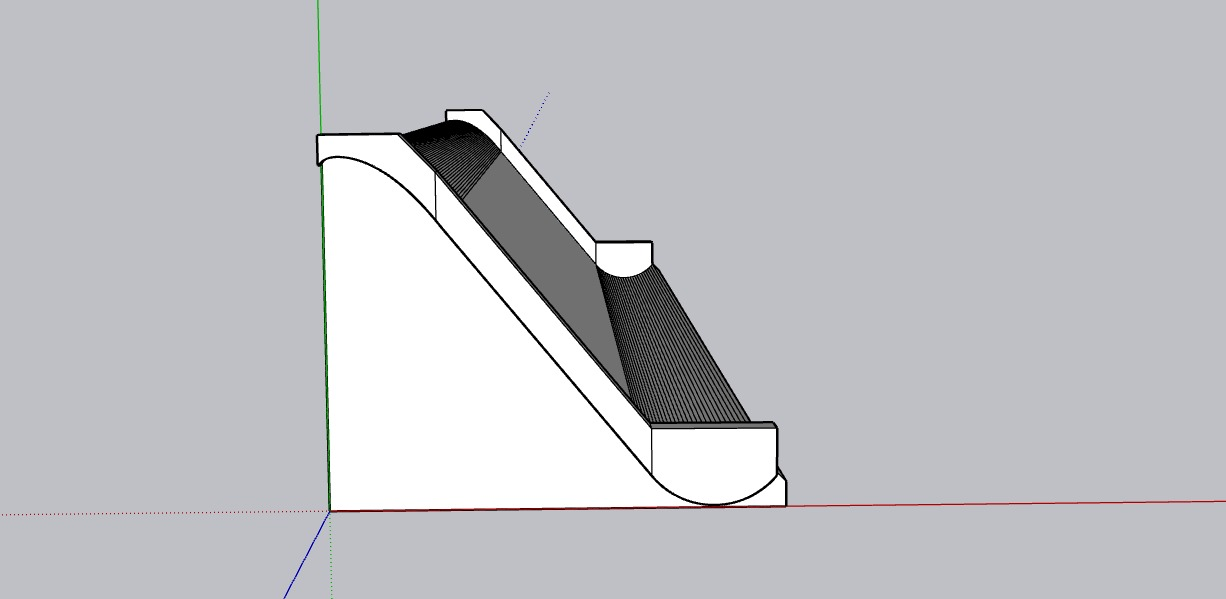
\includegraphics[width=0.85\textwidth]{figures/sketchup_domaine_calcul.jpeg}
    \caption{Modèle 3D SketchUp de l'évacuateur de crues du barrage Ahl Souss : vue en coupe du profil Creager, du coursier et de la cuillère de restitution, utilisé comme base de l'export STL pour la modélisation OpenFOAM.}
    \label{fig:domaine_calcul}
\end{figure}

La longueur totale du domaine de calcul a été fixée à \textbf{70 m}, depuis la face amont du réservoir jusqu'à l'extrémité aval de la zone d'impact, comme l'illustre la figure suivante :

\begin{figure}[H]
    \centering
    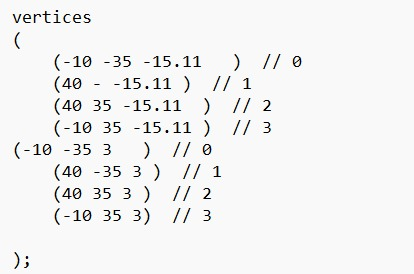
\includegraphics[width=\textwidth]{figures/ch8_domaine_70m.jpeg}
    \caption{Vue du domaine de calcul 3D sous OpenFOAM — longueur totale de 70\,m englobant la retenue amont, l'ouvrage (seuil Creager, coursier, cuillère) et la zone d'impact aval.}
    \label{fig:domaine_70m}
\end{figure}

Bien que la longueur totale de l'évacuateur soit de 70 m, les simulations de production ont été réalisées sur un domaine réduit de \textbf{20 m} dans la direction transversale. Ce choix se justifie par le caractère \textbf{homogène} de l'ouvrage : la géométrie (profil Creager, coursier, cuillère) est strictement identique en tout point de la largeur du barrage, de sorte que l'écoulement qui se développe sur une tranche de 20 m est en tous points représentatif de ce qui se produit sur l'ensemble des 70 m. Réduire le domaine à 20 m permet ainsi de diviser significativement le nombre de cellules du maillage et, par conséquent, le temps de calcul, sans introduire aucune approximation sur les résultats hydrauliques.

% SECTION : GÉNÉRATION DU MAILLAGE
\section{Génération du maillage}
\label{sec:generation_maillage}

\subsection{Initialisation du cas de simulation}
\label{subsec:initialisation_cas}

Avant de procéder à la génération du maillage, le cas OpenFOAM est initialisé en créant l'arborescence standard du répertoire de travail. La figure \ref{fig:dossier_initiation} présente la structure du dossier du cas, conforme à l'organisation décrite au chapitre \ref{chap:structure_cfd_openfoam} :

\begin{figure}[H]
    \centering
    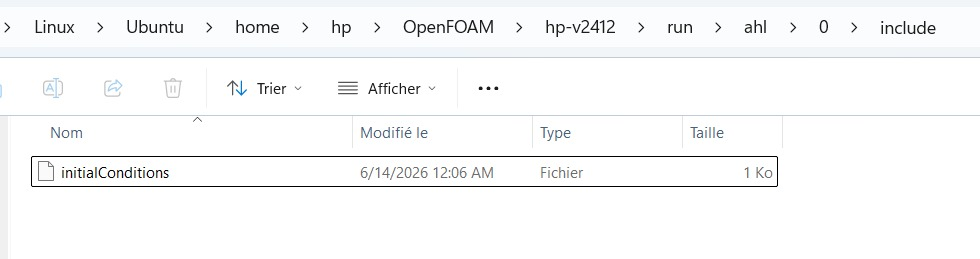
\includegraphics[width=0.70\textwidth]{figures/ch8_dossier_initiation.jpeg}
    \caption{Structure du dossier du cas OpenFOAM pour la simulation de l'évacuateur de crues — répertoires \texttt{0/}, \texttt{constant/} et \texttt{system/} avec leurs fichiers de configuration respectifs.}
    \label{fig:dossier_initiation}
\end{figure}

Le répertoire \texttt{0/} contient les fichiers décrivant les conditions initiales de chaque champ (\texttt{alpha.water}, \texttt{U}, \texttt{p\_rgh}, \texttt{k}, \texttt{omega}). La figure \ref{fig:condition_initiale} montre le contenu de ces fichiers d'initialisation :

\begin{figure}[H]
    \centering
    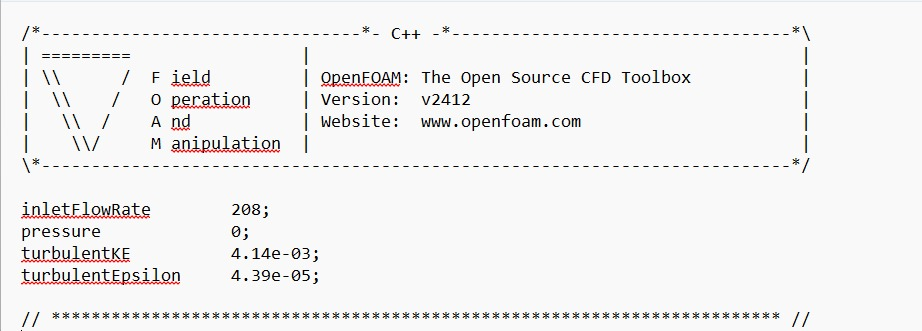
\includegraphics[width=\textwidth]{figures/ch8_condition_initiale.jpeg}
    \caption{Fichiers du répertoire \texttt{0/} du cas OpenFOAM — définition des conditions initiales des champs \texttt{alpha.water}, \texttt{U}, \texttt{p\_rgh} et des grandeurs de turbulence.}
    \label{fig:condition_initiale}
\end{figure}

Une fois les fichiers de conditions initiales en place, la commande \texttt{setFields} est exécutée pour initialiser les champs de manière cohérente avec la géométrie du domaine : le champ \texttt{alpha.water} est mis à 1 dans la zone du réservoir (eau) et à 0 dans la zone atmosphérique (air), en s'appuyant sur les régions de cellules définies dans \texttt{setFieldsDict}. La figure \ref{fig:setfields} illustre l'interface de cette commande :

\begin{figure}[H]
    \centering
    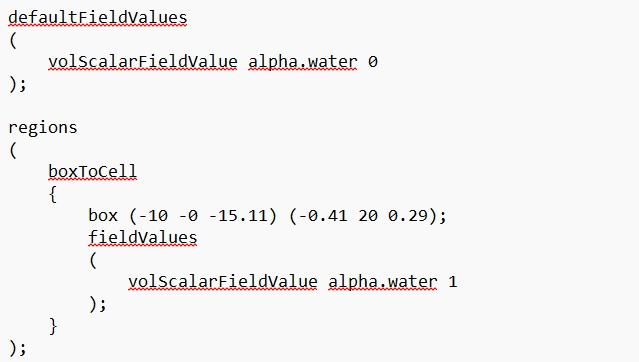
\includegraphics[width=\textwidth]{figures/ch8_setfields.jpeg}
    \caption{Exécution de la commande \texttt{setFields} — initialisation du champ \texttt{alpha.water} à 1 dans la zone de la retenue et à 0 dans la zone atmosphérique, conformément au fichier \texttt{system/setFieldsDict}.}
    \label{fig:setfields}
\end{figure}

Le profil de la surface libre initiale obtenu après l'exécution de \texttt{setFields}, visualisé sous ParaView, confirme que la répartition eau/air est correctement définie au démarrage de la simulation :

\begin{figure}[H]
    \centering
    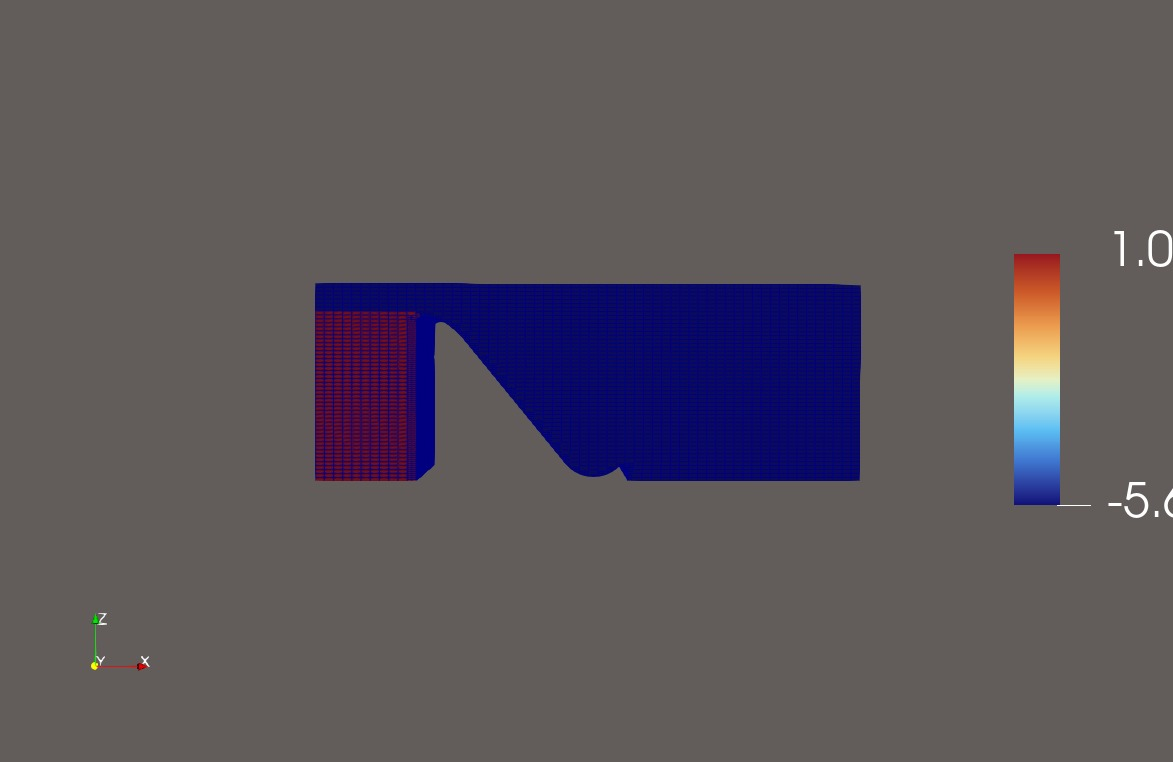
\includegraphics[width=\textwidth]{figures/ch8_profil_clair.jpeg}
    \caption{Profil de la surface libre initiale après \texttt{setFields} — visualisation du champ \texttt{alpha.water} (eau en bleu, air en blanc) à $t = 0$ dans ParaView ; le niveau d'eau dans la retenue correspond au niveau de la retenue normale.}
    \label{fig:profil_clair}
\end{figure}

\subsection{Maillage de base (blockMesh)}
\label{subsec:blockmesh}

La première étape de la génération du maillage consiste à définir, via l'utilitaire \texttt{blockMesh} et son fichier de configuration \texttt{blockMeshDict}, un maillage de fond hexaédrique englobant l'ensemble du domaine de calcul défini à la section \ref{sec:preparation_geometrie}. Ce maillage de base, relativement grossier, constitue le point de départ du raffinement effectué par \texttt{snappyHexMesh} \cite{greenshields2020openfoam, openfoam2022guide}.

Le maillage de fond obtenu après l'exécution de \texttt{blockMesh} est illustré par la figure suivante :

\begin{figure}[H]
    \centering
    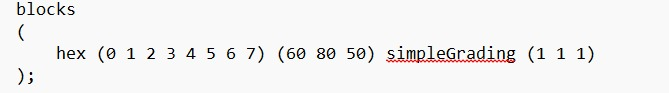
\includegraphics[width=\textwidth]{figures/ch8_maillage_grossier.jpeg}
    \caption{Vue d'ensemble du maillage de fond hexaédrique généré par \texttt{blockMesh} — maillage non raffiné couvrant l'intégralité du domaine de calcul (coupe verticale dans le plan médian de l'évacuateur).}
    \label{fig:maillage_global}
\end{figure}

\subsection{Raffinement et capture de la géométrie (snappyHexMesh)}
\label{subsec:snappyhexmesh}

L'utilitaire \texttt{snappyHexMesh} est ensuite utilisé pour adapter le maillage de fond aux surfaces STL importées (section \ref{sec:preparation_geometrie}), selon les trois étapes classiques \cite{greenshields2020openfoam} :
\begin{enumerate}
    \item \textbf{Castellation} : découpage des cellules du maillage de fond intersectant les surfaces STL ;
    \item \textbf{Snapping} : projection des points du maillage sur les surfaces STL pour reproduire fidèlement la géométrie de l'ouvrage (profil Creager, coursier, cuillère) ;
    \item \textbf{Ajout de couches limites (\textit{layers})} : insertion de couches de cellules fines au voisinage immédiat des parois solides, afin de mieux résoudre les gradients de vitesse dans la couche limite et d'atteindre une valeur de $y^+$ compatible avec les fonctions de paroi du modèle de turbulence retenu (section \ref{sec:conditions_limites}).
\end{enumerate}

Des zones de raffinement local (\texttt{refinementRegions} et \texttt{refinementSurfaces}) sont définies :
\begin{itemize}
    \item Au voisinage de l'\textbf{interface air-eau} (zone de battement du champ \texttt{alpha.water}), afin de limiter la diffusion numérique de l'interface et de capturer précisément la ligne d'eau le long du coursier ;
    \item Au voisinage du \textbf{seuil, du coursier et de la cuillère}, où les gradients de vitesse et de pression sont les plus marqués ;
    \item Le long de la \textbf{trajectoire théorique du jet} (section \ref{sec:distance_impact_jet}), pour assurer une résolution suffisante de la zone d'impact et de la fosse d'érosion (section \ref{sec:affouillement}).
\end{itemize}

Le fichier de configuration \texttt{snappyHexMeshDict} regroupe l'ensemble de ces paramètres de raffinement. La figure \ref{fig:snappyhexmeshdict} en présente un extrait :

\begin{figure}[H]
    \centering
    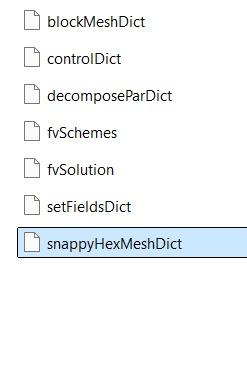
\includegraphics[height=0.55\textheight,keepaspectratio]{figures/ch8_snappyhexmeshdict.jpeg}
    \caption{Extrait du fichier \texttt{system/snappyHexMeshDict} — paramétrage des niveaux de raffinement par surface (\texttt{refinementSurfaces}) et par région (\texttt{refinementRegions}), ainsi que des paramètres de couches limites (\texttt{addLayersControls}).}
    \label{fig:snappyhexmeshdict}
\end{figure}

La qualité du maillage final est vérifiée à l'aide de l'utilitaire \texttt{checkMesh}, qui contrôle notamment la non-orthogonalité maximale, le \textit{skewness} et le rapport d'aspect des cellules \cite{knupp1993fundamentals}. Ces indicateurs doivent rester dans des plages compatibles avec la stabilité et la précision des schémas numériques du solveur \texttt{interFoam} (section \ref{sec:configuration_solveur}).

Le maillage raffiné obtenu après l'exécution de \texttt{snappyHexMesh} est présenté à la figure \ref{fig:maillage_detail} :

\begin{figure}[H]
    \centering
    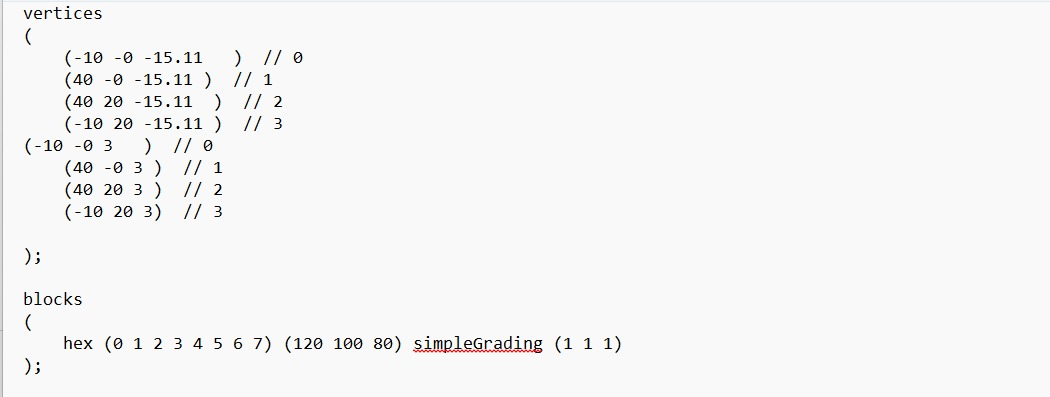
\includegraphics[width=\textwidth]{figures/ch8_maillage_raffine.jpeg}
    \caption{Vue rapprochée du maillage raffiné généré par \texttt{snappyHexMesh} au niveau du seuil Creager, du coursier et de la cuillère saut de ski — les couches de raffinement local et les couches limites sont clairement visibles au voisinage des parois solides.}
    \label{fig:maillage_detail}
\end{figure}

\subsection{Étude de sensibilité au maillage}
\label{subsec:sensibilite_maillage}

Afin de s'assurer que les résultats de la simulation sont indépendants de la résolution du maillage, une étude de sensibilité a été menée en comparant trois niveaux de raffinement (grossier, moyen, fin), construits en faisant varier le niveau de raffinement global et local de \texttt{snappyHexMesh} \cite{roache1998verification}. Pour chaque maillage, une grandeur de référence (par exemple la hauteur d'eau sur le coursier en une section donnée) est comparée entre les trois niveaux, afin de retenir le maillage offrant le meilleur compromis entre précision des résultats et coût de calcul.

Dans le cadre de cette étude, deux simulations ont été réalisées pour le débit millénal $Q_{1\,000} = 794{,}93$ m³/s :
\begin{itemize}
    \item \textbf{Simulation sur le domaine 70 m avec maillage non raffiné} : ce cas a d'abord été effectué pour visualiser l'écoulement sur la totalité de la structure. Le maillage utilisé est le maillage de fond grossier issu de \texttt{blockMesh} (figure \ref{fig:maillage_global}).
    \item \textbf{Simulation sur le domaine 20 m avec maillage raffiné} : ce cas constitue la simulation de référence. Le maillage est celui généré par \texttt{snappyHexMesh} avec raffinement local au niveau de l'ouvrage (figure \ref{fig:maillage_detail}).
\end{itemize}

La grandeur de comparaison est le champ \texttt{alpha.water} (fraction volumique d'eau), qui représente directement la position de la surface libre. Les profils \texttt{alpha.water} obtenus avec les deux configurations sont superposés : si les résultats concordent, la simulation sur 20 m avec maillage raffiné est validée et retenue pour l'ensemble de l'étude.


Les figures \ref{fig:alpha_70_grossier} et \ref{fig:alpha_20_raffine} présentent les champs \texttt{alpha.water} obtenus pour chacune des deux configurations, visualisés dans le plan médian longitudinal de l'évacuateur.

\begin{figure}[H]
    \centering
    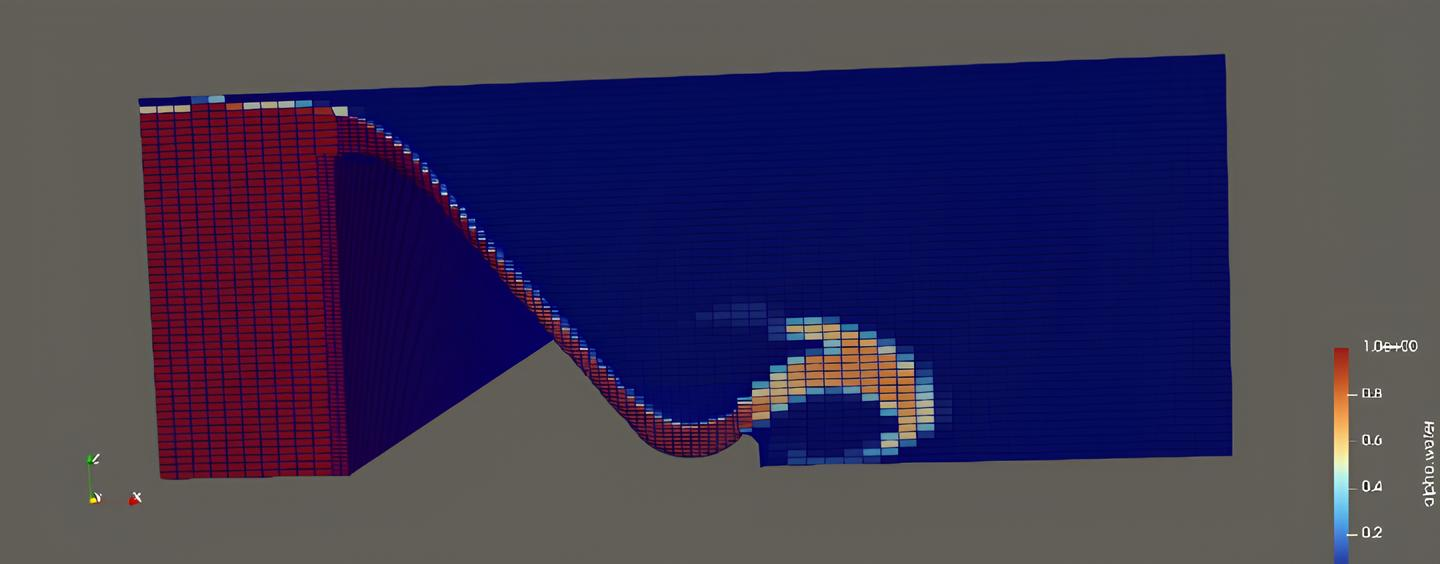
\includegraphics[width=\textwidth]{figures/ch8_alpha_70_grossier.jpeg}
    \caption{Champ \texttt{alpha.water} — domaine 70\,m avec maillage non raffiné (\texttt{blockMesh}), débit millénal $Q_{1\,000} = 794{,}93$ m³/s. La surface libre (interface eau/air) est visible mais sa définition reste approximative en raison de la faible résolution du maillage grossier.}
    \label{fig:alpha_70_grossier}
\end{figure}

\begin{figure}[H]
    \centering
    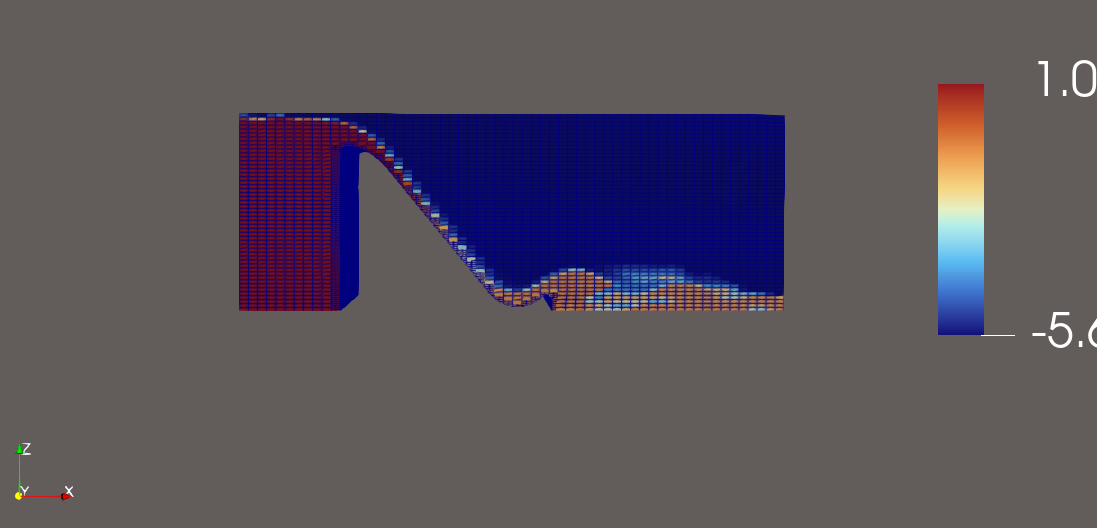
\includegraphics[width=\textwidth]{figures/ch8_alpha_20_raffine.png}
    \caption{Champ \texttt{alpha.water} — domaine 20\,m avec maillage raffiné (\texttt{snappyHexMesh}), débit millénal $Q_{1\,000} = 794{,}93$ m³/s. L'interface eau/air est nettement plus précise et la surface libre sur le coursier est bien capturée grâce au raffinement local.}
    \label{fig:alpha_20_raffine}
\end{figure}

La comparaison des deux champs \texttt{alpha.water} montre que les profils de la surface libre obtenus avec les deux configurations sont \textbf{en accord} : la position de l'interface eau/air, la hauteur d'eau sur le seuil et le long du coursier, ainsi que la trajectoire du jet en aval de la cuillère sont cohérents entre les deux simulations. La simulation sur le domaine réduit de 20 m avec maillage raffiné reproduit donc fidèlement les résultats du domaine complet de 70 m, tout en offrant une résolution spatiale nettement supérieure au niveau de l'ouvrage.

\bigskip
Afin de renforcer cette validation, le \textbf{champ de vitesse U} a également été comparé entre les deux configurations. La distribution spatiale des vitesses constitue en effet un indicateur sensible de la qualité du maillage : un maillage insuffisamment raffiné tend à lisser les gradients de vitesse, à sous-estimer les vitesses maximales au voisinage des parois et à mal reproduire la structure de l'écoulement dans les zones de forte courbure (seuil, cuillère).

\begin{figure}[H]
    \centering
    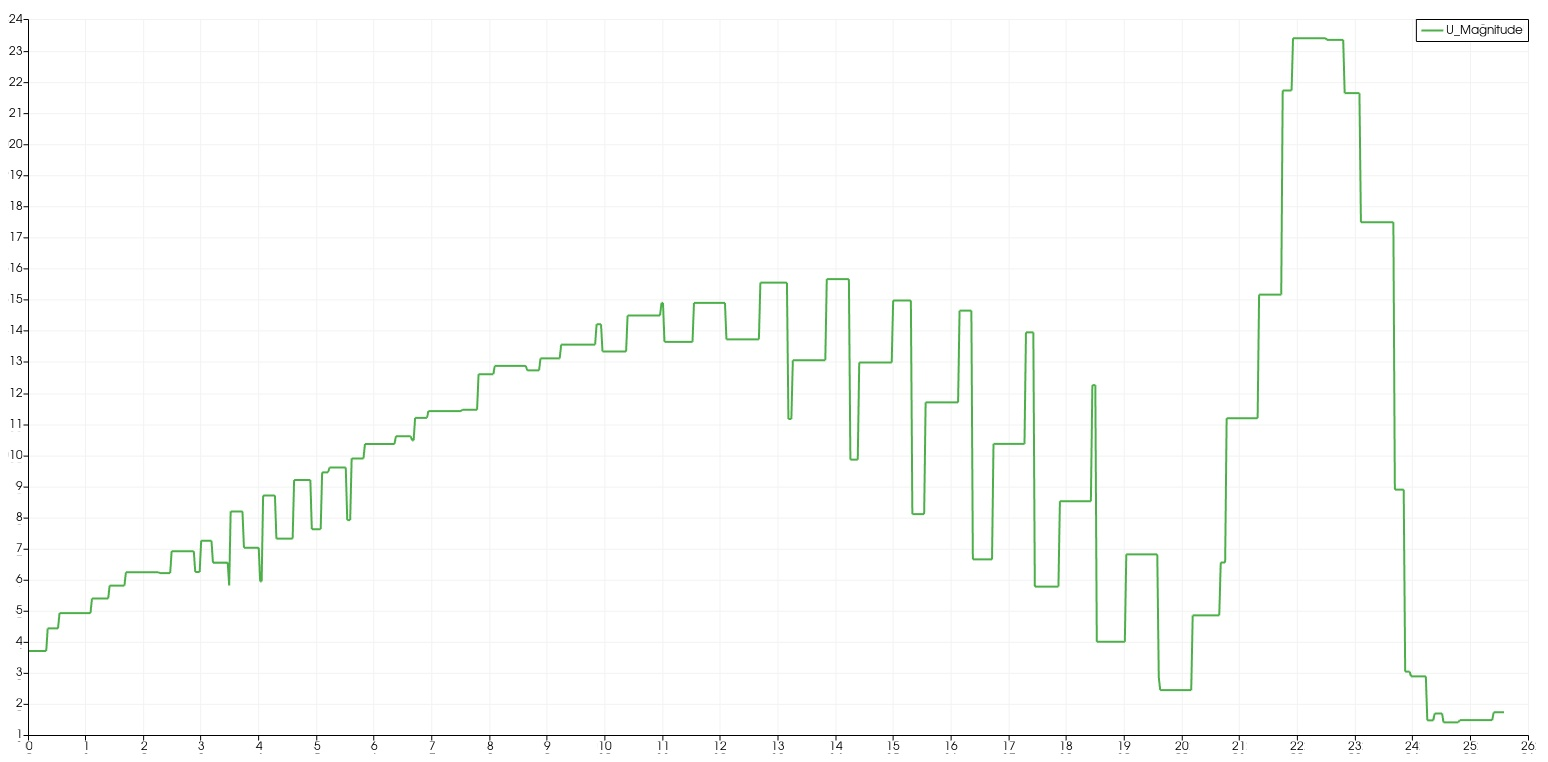
\includegraphics[width=\textwidth]{figures/ch8_U_70_grossier.jpeg}
    \caption{Champ de vitesse $\|\mathbf{U}\|$ (m/s) — domaine 70\,m avec maillage non raffiné (\texttt{blockMesh}), débit millénal $Q_{1\,000} = 794{,}93$ m³/s. Les gradients de vitesse sont peu résolus et la distribution apparaît homogène par excès de diffusion numérique due à la grande taille des cellules.}
    \label{fig:U_70_grossier}
\end{figure}

\begin{figure}[H]
    \centering
    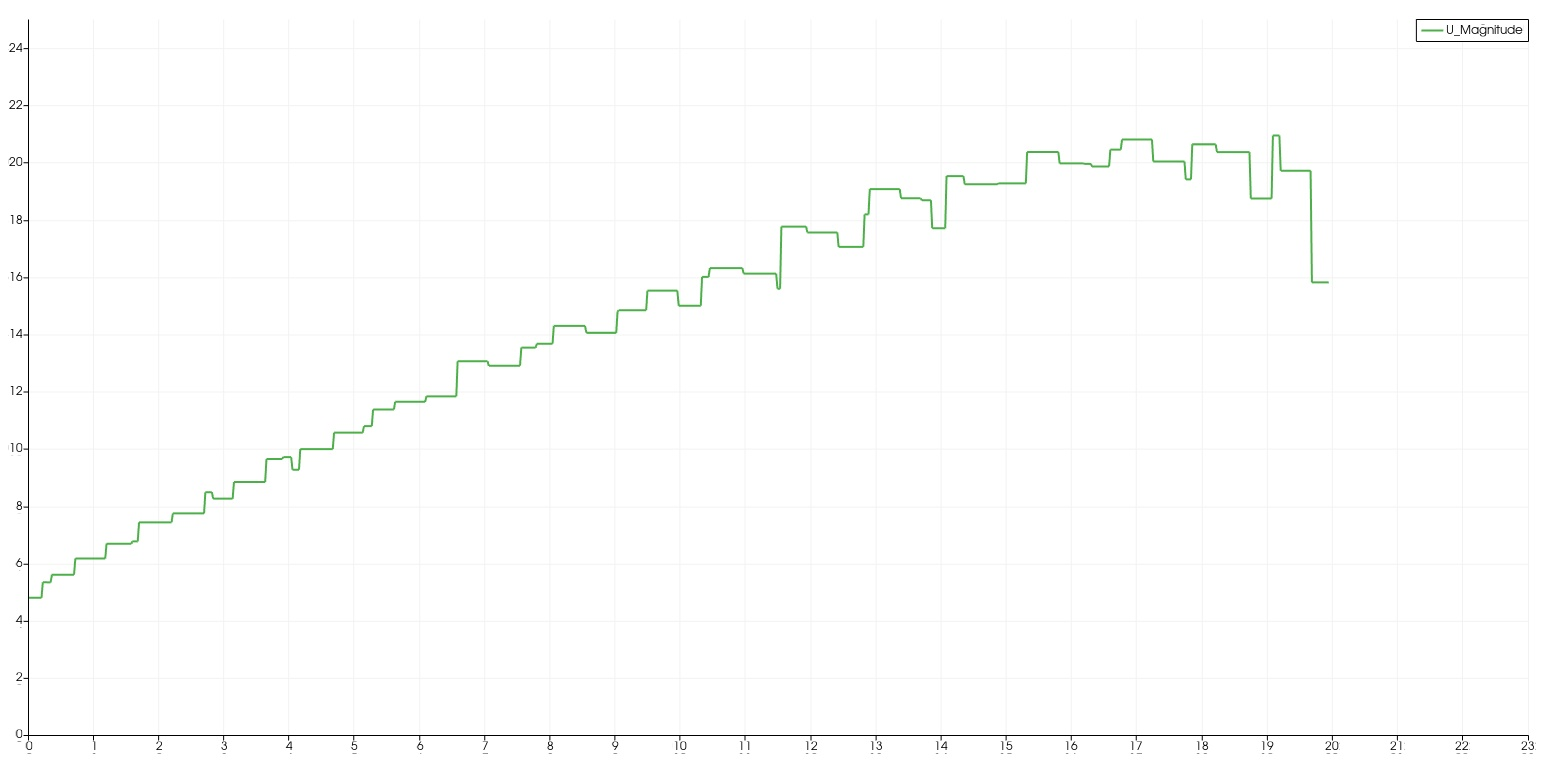
\includegraphics[width=\textwidth]{figures/ch8_U_20_raffine.jpeg}
    \caption{Champ de vitesse $\|\mathbf{U}\|$ (m/s) — domaine 20\,m avec maillage raffiné (\texttt{snappyHexMesh}), débit millénal $Q_{1\,000} = 794{,}93$ m³/s. Les gradients de vitesse sont nettement mieux résolus : l'accélération de l'écoulement sur le seuil Creager, les vitesses élevées sur le coursier et la distribution du jet en aval de la cuillère sont clairement visibles.}
    \label{fig:U_20_raffine}
\end{figure}

La comparaison des deux champs de vitesse met en évidence l'apport du raffinement du maillage :
\begin{itemize}
    \item Sur le \textbf{maillage grossier} (70 m), les gradients de vitesse sont diffus et les vitesses maximales sont sous-estimées ; la structure de l'écoulement au niveau du seuil et de la cuillère est imprécise.
    \item Sur le \textbf{maillage raffiné} (20 m), les vitesses sont bien résolues, les zones d'accélération et de décélération sont nettement distinguées, et la distribution transversale de l'écoulement est cohérente avec les résultats théoriques du chapitre \ref{chap:dimensionnement_theorique}.
\end{itemize}

L'accord global entre les champs \texttt{alpha.water} et les champs de vitesse des deux configurations confirme la \textbf{convergence en maillage} de la solution : le maillage raffiné sur 20 m capture correctement la physique de l'écoulement et constitue un choix pertinent pour l'ensemble des simulations de production présentées au chapitre \ref{chap:resultats_simulation}.

Le maillage retenu pour l'ensemble des simulations présentées dans ce rapport est celui offrant un écart négligeable sur la grandeur de référence par rapport au maillage le plus fin, pour un coût de calcul maîtrisé.

\subsection{Visualisation du maillage sous ParaView}
\label{subsec:visualisation_paraview}

La géométrie maillée est chargée sous \textbf{ParaView} en ouvrant le fichier \texttt{ahl.foam} généré dans le répertoire du cas. Cette opération permet de vérifier visuellement la cohérence du maillage avec la géométrie STL importée, et de contrôler la qualité du raffinement au voisinage de l'ouvrage.

\begin{figure}[H]
    \centering
    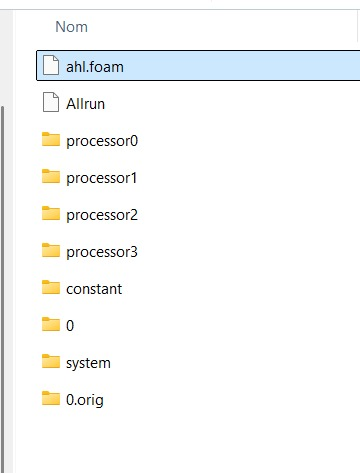
\includegraphics[height=0.55\textheight,keepaspectratio]{figures/ch8_paraview_ahl.jpeg}
    \caption{Ouverture du cas OpenFOAM dans ParaView via le fichier \texttt{ahl.foam} — la géométrie complète de l'évacuateur de crues (profil Creager, coursier, cuillère) apparaît correctement chargée avec son maillage raffiné.}
    \label{fig:paraview_ahl}
\end{figure}

\begin{figure}[H]
    \centering
    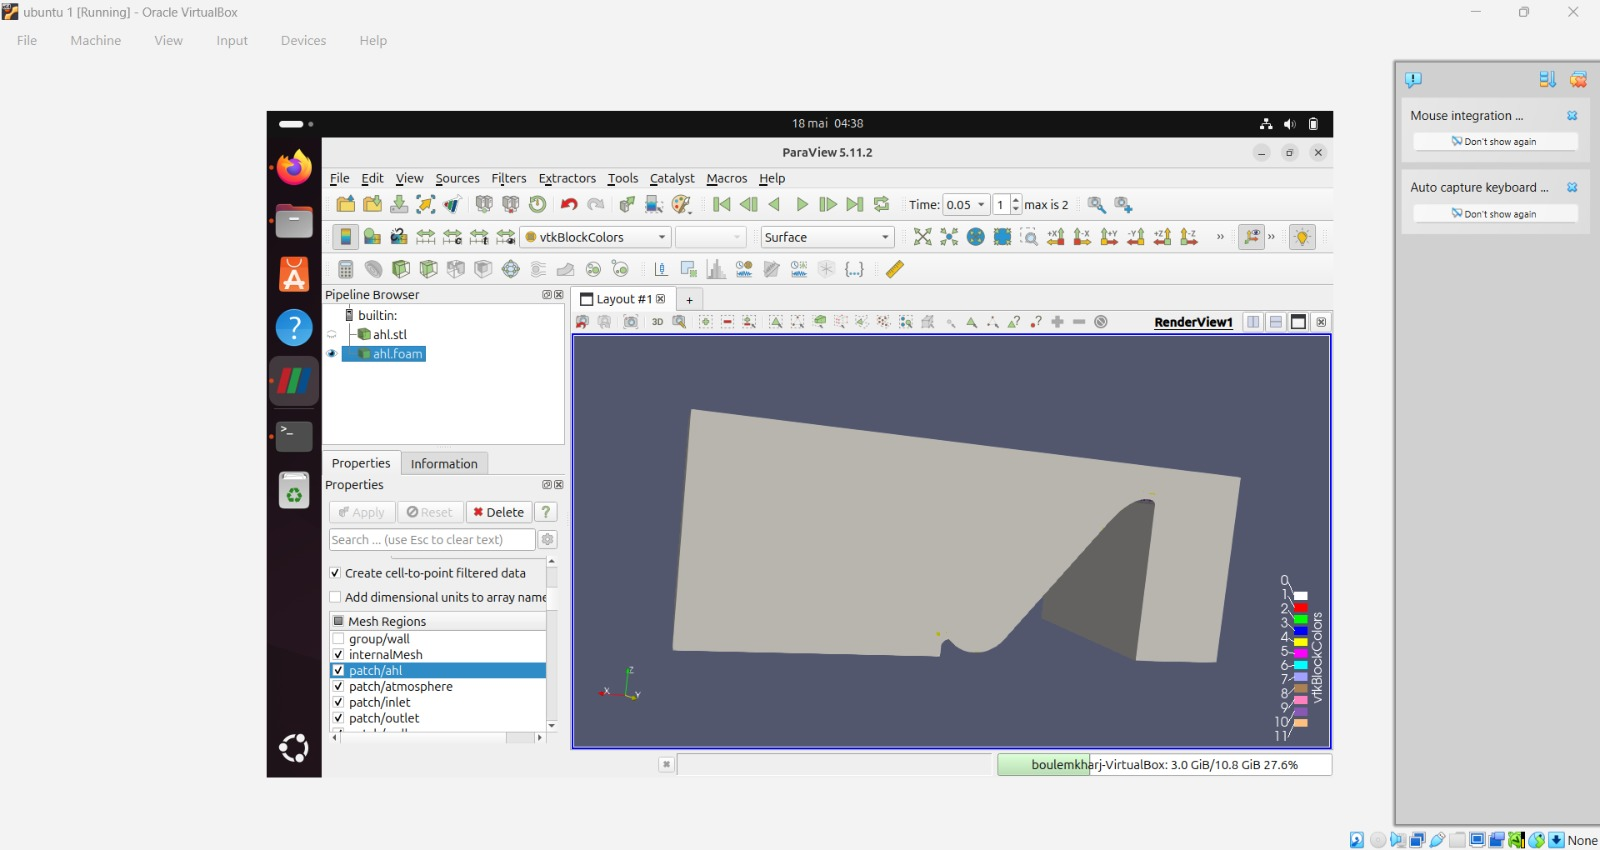
\includegraphics[width=\textwidth]{figures/ch8_paraview1.jpeg}
    \caption{Visualisation du maillage de l'évacuateur de crues sous ParaView (vue 1) — vue d'ensemble du domaine de calcul montrant la répartition des cellules du maillage et les zones de raffinement local.}
    \label{fig:paraview1}
\end{figure}


% SECTION : CONDITIONS INITIALES ET AUX LIMITES
\section{Conditions initiales et conditions aux limites}
\label{sec:conditions_limites}

\subsection{Conditions initiales}
\label{subsec:conditions_initiales}

À l'instant initial ($t=0$), le domaine de calcul est initialisé à l'aide de l'utilitaire \texttt{setFields}, selon les principes suivants :
\begin{itemize}
    \item Le champ \texttt{alpha.water} est initialisé à 1 dans la portion du domaine située sous le niveau d'eau correspondant au débit simulé (niveau de retenue normale $Z = 600{,}00$ NGM majoré de la charge $H$ du tableau \ref{tab:loi_debit_charge}), et à 0 ailleurs (zone atmosphérique et coursier initialement sec) ;
    \item Le champ de pression \texttt{p\_rgh} est initialisé de manière hydrostatique, cohérent avec la répartition initiale du champ \texttt{alpha.water} ;
    \item Le champ de vitesse \texttt{U} est initialisé à $\mathbf{0}$ (eau initialement au repos), l'écoulement se développant progressivement sous l'effet du déversement sur le seuil ;
    \item Les champs de turbulence \texttt{k} et \texttt{omega} sont initialisés à des valeurs uniformes faibles, estimées à partir d'une intensité turbulente caractéristique et d'une longueur de mélange représentative de la géométrie de l'écoulement \cite{menter1994two}.
\end{itemize}

\subsection{Conditions aux limites}
\label{subsec:conditions_aux_limites}

Les conditions aux limites sont définies pour chaque frontière (\textit{patch}) du domaine de calcul, en cohérence avec les types de conditions présentés au chapitre \ref{chap:structure_cfd_openfoam} (tableau \ref{tab:boundary_conditions}). Le tableau \ref{tab:cl_ahl_souss} synthétise les conditions retenues pour les principaux champs (\texttt{alpha.water}, \texttt{U}, \texttt{p\_rgh}, \texttt{k}, \texttt{omega}) sur chacune des frontières du domaine.

\begin{table}[H]
    \centering
    \caption{Conditions aux limites retenues pour le cas Ahl Souss}
    \label{tab:cl_ahl_souss}
    \resizebox{\textwidth}{!}{%
    \begin{tabular}{|l|c|c|c|c|c|}
        \hline
        \textbf{Frontière} & \textbf{\texttt{alpha.water}} & \textbf{\texttt{U}} & \textbf{\texttt{p\_rgh}} & \textbf{\texttt{k} / \texttt{omega}} & \textbf{Remarque} \\
        \hline
        Amont (réservoir) & \texttt{fixedValue} & \texttt{pressureInletOutletVelocity} & \texttt{totalPressure} & \texttt{fixedValue} & Niveau d'eau imposé selon $Q$ \\
        \hline
        Aval (sortie) & \texttt{inletOutlet} & \texttt{pressureInletOutletVelocity} & \texttt{totalPressure} & \texttt{inletOutlet} & Sortie libre \\
        \hline
        Atmosphère (haut) & \texttt{inletOutlet} & \texttt{pressureInletOutletVelocity} & \texttt{totalPressure} & \texttt{inletOutlet} & Pression atmosphérique \\
        \hline
        Parois (fond, ouvrage) & \texttt{zeroGradient} & \texttt{noSlip} & \texttt{fixedFluxPressure} & \texttt{kqRWallFunction} / \texttt{omegaWallFunction} & Fonctions de paroi, $k-\omega$ SST \\
        \hline
        Plans latéraux & \texttt{zeroGradient} & \texttt{slip} ou \texttt{symmetry} & \texttt{zeroGradient} / \texttt{symmetry} & \texttt{symmetry} & Selon configuration retenue \\
        \hline
    \end{tabular}}
\end{table}

Le modèle de turbulence retenu est le modèle $k-\omega$ SST de Menter \cite{menter1994two}, déjà présenté au chapitre \ref{chap:turbulence} (section \ref{subsec:modele_k_omega_sst}), qui offre un bon compromis entre robustesse et précision pour les écoulements à surface libre comportant à la fois des zones de proche paroi et des zones de cisaillement libre (jet, surface libre) \cite{moukalled2016finite}.

% SECTION : CONFIGURATION DU SOLVEUR INTERFOAM
\section{Configuration du solveur interFoam}
\label{sec:configuration_solveur}

\subsection{Schémas de discrétisation (fvSchemes)}
\label{subsec:fvschemes}

Le fichier \texttt{fvSchemes} définit les schémas numériques utilisés pour discrétiser les différents termes des équations résolues par \texttt{interFoam} \cite{rusche2002computational} :
\begin{itemize}
    \item \textbf{Schéma temporel (\texttt{ddtSchemes})} : schéma \texttt{Euler}, implicite du premier ordre, adapté au pas de temps variable utilisé en régime transitoire ;
    \item \textbf{Schémas de gradient (\texttt{gradSchemes})} : schéma \texttt{Gauss linear}, du second ordre ;
    \item \textbf{Schémas de divergence (\texttt{divSchemes})} : un schéma de type \texttt{vanLeer}, borné et peu diffusif, est utilisé pour l'advection du champ \texttt{alpha.water} (méthode MULES) afin de préserver la netteté de l'interface air-eau ; des schémas de type \texttt{linearUpwind} ou \texttt{limitedLinear} sont utilisés pour le terme convectif de \texttt{U} et pour les équations de turbulence ($k$, $\omega$), afin de garantir la stabilité du calcul ;
    \item \textbf{Schémas laplaciens (\texttt{laplacianSchemes})} : schéma \texttt{Gauss linear corrected}, avec correction de non-orthogonalité ;
    \item \textbf{Schémas d'interpolation} : interpolation linéaire entre centres de cellules et faces.
\end{itemize}

\subsection{Paramètres de résolution (fvSolution) et algorithme PIMPLE}
\label{subsec:fvsolution}

Le fichier \texttt{fvSolution} définit les solveurs linéaires et leurs critères de convergence pour chaque champ, ainsi que les paramètres de l'algorithme de couplage pression-vitesse \cite{holzmann2017mathematics} :
\begin{itemize}
    \item Le champ \texttt{alpha.water} est résolu par la méthode \textbf{MULES} (\textit{Multidimensional Universal Limiter with Explicit Solution}), avec un nombre de sous-cycles (\texttt{nAlphaSubCycles}) et un coefficient de compression d'interface (\texttt{cAlpha}) permettant de limiter la diffusion numérique de l'interface air-eau ;
    \item Le champ de pression \texttt{p\_rgh} est résolu par un solveur de type \texttt{GAMG} (\textit{Geometric-Algebraic Multi-Grid}) ou \texttt{PCG} avec préconditionneur \texttt{DIC} ;
    \item Les champs \texttt{U}, \texttt{k} et \texttt{omega} sont résolus par un solveur de type \texttt{smoothSolver} ou \texttt{PBiCG} avec préconditionneur \texttt{DILU} ;
    \item L'algorithme \textbf{PIMPLE} (chapitre \ref{chap:structure_cfd_openfoam}, section \ref{subsec:pimple}) est configuré avec un nombre de correcteurs externes (\texttt{nOuterCorrectors}), un nombre de correcteurs de pression (\texttt{nCorrectors}) et un nombre de correcteurs de non-orthogonalité (\texttt{nNonOrthogonalCorrectors}) adaptés à la qualité du maillage (section \ref{subsec:sensibilite_maillage}) ;
    \item Des facteurs de sous-relaxation sont appliqués sur la pression et la vitesse au sein des itérations externes, afin de stabiliser la convergence à chaque pas de temps.
\end{itemize}


% SECTION : LANCEMENT DES SIMULATIONS ET CONVERGENCE
\section{Lancement des simulations et suivi de la convergence}
\label{sec:lancement_simulations}

\subsection{Campagne de simulations}
\label{subsec:campagne_simulations}

Conformément aux objectifs de l'étude, une simulation a été réalisée pour chacun des trois débits laminés du tableau \ref{tab:debits_lamines} (périodes de retour 10, 100 et 1\,000 ans), avec un maillage et une configuration de solveur identiques (sections \ref{sec:generation_maillage} et \ref{sec:configuration_solveur}), seule la condition à la limite amont (niveau d'eau / débit imposé) variant d'une simulation à l'autre. Un scénario complémentaire, correspondant à une surélévation hypothétique du plan d'eau de 1 m, est traité séparément à titre de supplément (chapitre \ref{chap:resultats_simulation}, section \ref{sec:supplement_surelevation}).

Les calculs ont été exécutés en parallèle à l'aide de la décomposition de domaine (\texttt{decomposePar}), selon une méthode de décomposition de type \textit{scotch}, répartissant le maillage sur plusieurs cœurs de calcul afin de réduire le temps de restitution.

La figure \ref{fig:decomposePar} illustre la configuration du fichier \texttt{decomposeParDict} utilisé pour la décomposition du domaine, et la figure \ref{fig:decomposePar_result} montre les répertoires générés après l'exécution de \texttt{decomposePar} :

\begin{figure}[H]
    \centering
    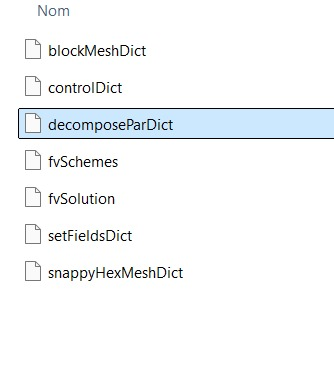
\includegraphics[width=\textwidth]{figures/ch8_decomposePar.jpeg}
    \caption{Configuration de la décomposition de domaine dans le fichier \texttt{system/decomposeParDict} — méthode \textit{scotch} avec répartition automatique du maillage entre les processeurs.}
    \label{fig:decomposePar}
\end{figure}

\begin{figure}[H]
    \centering
    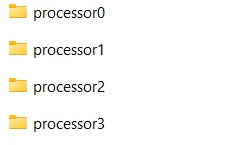
\includegraphics[width=\textwidth]{figures/ch8_decomposePar_result.jpeg}
    \caption{Répertoires créés par la commande \texttt{decomposePar} — chaque sous-répertoire \texttt{processor\textit{N}/} contient la portion du maillage et des champs attribuée au processeur \textit{N} pour le calcul parallèle.}
    \label{fig:decomposePar_result}
\end{figure}

\subsection{Suivi de la convergence}
\label{subsec:suivi_convergence}

La convergence et la stabilité de chaque simulation sont contrôlées tout au long du calcul à l'aide des indicateurs suivants :
\begin{itemize}
    \item Les \textbf{résidus} des champs \texttt{p\_rgh}, \texttt{Ux}, \texttt{Uy} et \texttt{Uz}, dont la décroissance traduit la convergence de la résolution à chaque pas de temps ;
    \item Le \textbf{nombre de Courant} (\texttt{Courant Number}), global et maximal, qui doit rester compatible avec les bornes \texttt{maxCo} et \texttt{maxAlphaCo} définies dans le fichier \texttt{controlDict} ;
    \item Les \textbf{erreurs de conservation de la masse} (\textit{continuity errors}), rapportées par \texttt{interFoam} à chaque pas de temps, qui doivent rester négligeables ;
    \item L'évolution temporelle de grandeurs physiques en des points de contrôle (sondes), telles que la hauteur d'eau ou la vitesse en une section donnée du coursier, dont la stabilisation traduit l'atteinte d'un régime quasi-permanent.
\end{itemize}

